\documentclass{exam}
\usepackage[utf8]{inputenc}
\usepackage{lmodern}
\usepackage{microtype}

% \usepackage[parfill]{parskip}
\usepackage[dvipsnames]{xcolor}
\usepackage{amsmath}
\usepackage{amsfonts}
\usepackage{amsthm}
\usepackage{siunitx}
\DeclareSIUnit\year{yr}
\DeclareSIUnit\foot{ft}
\DeclareSIUnit\litre{\liter}

\usepackage{skull}

\usepackage{pgfplots}
\usepgfplotslibrary{polar}
\pgfplotsset{compat=1.11}
\usepgfplotslibrary{statistics}
\usepackage{graphicx}
\usepackage{sidecap}
\sidecaptionvpos{figure}{c}
\usepackage{float}
\usepackage{gensymb}
\usepackage{tkz-euclide}
\usetkzobj{all}
\usepackage{commath}
\usepackage{hyperref}
\usepackage{enumitem}
\usepackage{wasysym}
\usepackage{multicol}
\usepackage{mathtools}
\usepackage{tcolorbox}
\usepackage{tabularx}
\usepackage[version=4]{mhchem}
\usepackage{changepage}
\usepackage{listings}
\lstset{basicstyle=\ttfamily\linespread{0.8}\small}

\renewcommand*{\thefootnote}{\fnsymbol{footnote}}

\newtheorem*{thm}{Theorem}
\newtheorem*{iden}{Identity}
\newtheorem*{lemma}{Lemma}
\newtheorem{obs}{Observation}
\theoremstyle{definition}
\newtheorem*{defn}{Definition}
\newtheorem*{ex}{Example}
\newtheorem{con}{Construction}
\newtheorem*{alg}{Algorithm}

\newtheoremstyle{break}
  {\topsep}{\topsep}%
  {\itshape}{}%
  {\bfseries}{}%
  {\newline}{}%
\theoremstyle{break}
\newtheorem*{bthm}{Theorem}

% russian integral
\usepackage{scalerel}
\DeclareMathOperator*{\rint}{\scalerel*{\rotatebox{17}{$\!\int\!$}}{\int}}

% \DeclareMathOperator*{\rint}{\int}

\pgfplotsset{vasymptote/.style={
    before end axis/.append code={
        \draw[densely dashed] ({rel axis cs:0,0} -| {axis cs:#1,0})
        -- ({rel axis cs:0,1} -| {axis cs:#1,0});
    }
}}

% \pointsinrightmargin
\boxedpoints
\pointname{}

\newcommand{\questioA}{\question[\texttt{\textbf{\color{Cerulean} A}}]}
\newcommand{\questioM}{\question[\texttt{\textbf{\color{PineGreen} M}}]}
\newcommand{\questioE}{\question[\texttt{\textbf{\color{WildStrawberry} E}}]}
\newcommand{\questioS}{\question[\texttt{\textbf{\color{Goldenrod} S}}]}
\newcommand{\questioO}{\question[\texttt{\textbf{\color{BurntOrange} O}}]}

\newcommand{\parA}{\part[\texttt{\textbf{\color{Cerulean} A}}]}
\newcommand{\parM}{\part[\texttt{\textbf{\color{PineGreen} M}}]}
\newcommand{\parE}{\part[\texttt{\textbf{\color{WildStrawberry} E}}]}
\newcommand{\parS}{\part[\texttt{\textbf{\color{Goldenrod} S}}]}
\newcommand{\parO}{\part[\texttt{\textbf{\color{BurntOrange} O}}]}

\newcommand{\subparA}{\subpart[\texttt{\textbf{\color{Cerulean} A}}]}
\newcommand{\subparM}{\subpart[\texttt{\textbf{\color{PineGreen} M}}]}
\newcommand{\subparE}{\subpart[\texttt{\textbf{\color{WildStrawberry} E}}]}
\newcommand{\subparS}{\subpart[\texttt{\textbf{\color{Goldenrod} S}}]}
\newcommand{\subparO}{\subpart[\texttt{\textbf{\color{BurntOrange} O}}]}

\newcommand{\mainHeader}[2]{\section*{NCEA Level 2 Mathematics\\#1. #2}}
\newcommand{\mainHeaderHw}[2]{\section*{NCEA Level 2 Mathematics (Homework)\\#1. #2}}
\newcommand{\seealso}[1]{\begin{center}\emph{See also #1.}\end{center}}
\newcommand{\drills}[1]{\begin{center}\emph{Drill problems: #1.}\end{center}}
\newcommand{\basedon}[1]{\begin{center}\emph{Notes largely based on #1.}\end{center}}

\begin{document}

\mainHeaderIntgHw{23}{Trigonometric Substitution}
\subsection*{Reading}
\begin{center}
  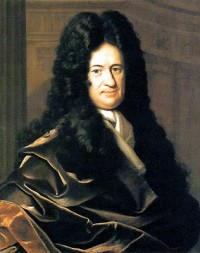
\includegraphics[height=0.2\textheight]{leibniz}
\end{center}

Whereas Newton had concentrated on finding the derivatives of given functions and on the inverse process, the recognition
that limits of sums like those in definite integrals can be obtained by reversing differentiation is due primarily to
Gottfried Wilhelm Leibniz (1646--1716). Leibniz' career contrasts sharply with Newton's. Newton had undertaken the study
of mathematics and physics early in life and had pursued these two fields almost exclusively, although he did make minor
contributions to chemistry and theology. His career as a professor gave him the opportunity to concentrate. Leibniz started
by studying law at the University of Leipzig, the city in which he grew up. He secured a doctor's degree in law at the
University of Altdorf in 1666. His first position was that of ambassador for the Elector of Mainz, and until 1672 his interest
in mathematics was secondary. In 1672, during a trip to Paris, he met Huygens (the astronomer and mathematician), who acquanted
Leibniz with current scientific problems and activities. Leibniz's interests were deeply stirred, and thereafter he devoted
much time to mathematics.

What is amazing about Leibniz is the vast quantity of first-rate contributions he made to other fields. Although his profession
was law, his work in mathematics and philosophy ranks among the best the world has produced. He also did major work in mechanics,
nautical science, optics, hydrostatics, logic, philology, geology, and theology, and was a pioneer in historical research. No
subject pursued by intellectuals of his age was neglected; only Leibniz himself went unrecognised and neglected by his contemporaries.

\begin{flushright}
  Adapted from \textit{Mathematics for the nonmathematician} (pp.406--7) by Morris Kline (Dover, 1985).
\end{flushright}

\subsection*{Questions}
Compute the following integrals. Some may not require trig substitution.
\begin{multicols}{2}
\begin{questions}
  \question $ \displaystyle\rint \frac{\dif{x}}{\sqrt{x^2 + 4}} $
  \question $ \displaystyle\rint \frac{x^6}{\sqrt{1 - x^{14}}} \dif{x} $
  \question $ \displaystyle\rint \sqrt{9 - x^2} \dif{x} $
  \question $ \displaystyle\rint x \sqrt{25x^2 - 4} \dif{x} $
  \question $ \displaystyle\rint \sqrt{4-9z^2} \dif{z} $
  \question $ \displaystyle\rint^{1/6}_0 \frac{x^5}{\left( 36x^2 + 1 \right)^{3/2}} \dif{x} $
  \question $ \displaystyle\rint \frac{\ln x}{x^5} \dif{x} $
  \question $ \displaystyle\rint^2_1 \frac{5t - 2}{2t^2 - t - 1} \dif{t} $
\end{questions}
\end{multicols}
\end{document}

